\documentclass[11pt]{article}

\usepackage[margin=0.75in]{geometry}
\usepackage{url}
\usepackage{graphicx}
\graphicspath{ {figs/} }

\title{An Analysis of fcMRI data in Schizophrenia}
\author{
  Hejazi, Nima\\
  \texttt{nhejazi}
  \and
  Lin, Feng\\
  \texttt{LiamFengLin}
  \and
  Zhao, Luyun\\
  \texttt{lynnzhao92}
  \and
  Zhou, Xinyue\\
  \texttt{z357412526}
}

\bibliographystyle{siam}

\begin{document}
\maketitle

\abstract{We report analyses intended to explore the functional magnetic
  resonance imaging (fMRI) data collected in studies conducted by Repovs et al.,
on the manner in which brain network connectivity is related to schizophrenia
\cite{repovs2011,repovs2012}. A host of exploratory analyses, combining both
classical linear modeling methods and machine learning, were undertaken in order
to gain further insights into the fMRI data examined.}

\section{Introduction}

The human central nervous system is a complex dynamic network, consisting of
numerous functional regions that coordinate everything from simple behaviors to
complicated thoughts. In an effort to better understand the manner in which
functional changes contribute to the symptoms of schizophrenia, Repovs \textit{et
al.} conducted neuroimaging studies, including both functional connectivity
magnetic resonance imaging (fcMRI) and diffusion tensor imaging (DTI), on many
subjects, with their goal being to characterize the activity of several brain
regions chosen a priori, and to develop an understanding of how the functional 
activities of these regions may differ across health states \cite{repovs2011,repovs2012}.

\section{Data}

The analyses reported in this paper are based on data generated in a series of
neuroimaging experiments conducted by Barch, Repovs, \& Csernansky. The aim of
these experiments was to ascertain the activity of several brain networks
thought to be associated with depressed cognitive function in individuals with
schizophrenia by collecting functional connectivity magnetic resonance imaging
(fcMRI) data on healthy individuals, individuals with schizophrenia, and the
(healthy) siblings of participants in either of the two former groups
\cite{repovs2012}. For the purposes of the analyses reported in this paper, the imaging
data were acquired from the OpenfMRI project (\url{https://openfmri.org/}), where they
are listed with accession number ds000115. The data is available for groups of
subjects, with each subject-specific data directory containing anatomical MR
imaging data, functional MR imaging (using the BOLD contrast) data, and
diffusion tensor imaging (DTI) data. In this preliminary report, the analyses
are restricted to the BOLD functional MR imaging data, for 8 subjects among
the pool of 102 subjects for which data are available, with most analyses
(ranging from linear modeling to machine learning with K-Means) taking the form
of exploratory examinations into the structure of this imaging data.

\section{Methods}

Literature notes that different regions of the brain exhibit different levels
and patterns of activities during performance of cognitive tasks
\cite{fox2005}. Some regions are associated with marked increase in
activities and some with decrease in activities. They are often given \textit{a priori}
in papers. One of the goals of our analysis is to identify activation regions
during the performance of n-back tasks using unsupervised learning methods
(e.g., K-Means), comparing the regions isolated in this manner with those
assumed in the literature. Specifically, we want to find regions that are
associated with dynamic, task-related and functional aspects of brain
activities, instead of just anatomical subdivisions. Two preliminary types of
analysis are performed and introduced below, along with diagnostic checks of the
validity of the results. 

\section{Results}

\subsection{Data Fetching and Preprocessing}

For all BOLD datasets, we removed the first five images to allow signals to
achieve steady state. In addition, we prepared scripts to detect the root mean
square (RMS) difference outliers using the Inter-Quartile Range (IQR) to define
outliers. This is because they could imply a sudden widespread shift in signals
caused by hardware issues. We have run all the analysis with the outliers
removed so far, but will run a portion of the analysis with the outliers in the
future and discuss the impact of excluding outliers. 

Some preprocessing tasks are analysis-specific. As will be discussed in a later
section, we scaled BOLD signals per time step to use them as one of the
feature sets for k-means clustering. 

\subsection{Correlations with Baseline Functions}

This set of methods aim to produce an image identifying the regions which show
significant signal change in response to the task by calculating correlation
coefficients (r) between the bold signal along the time course and a reference
waveform, for each voxel. A high value of the correlation coefficient means that
fluctuation of the signal in the locale of the brain is task-dependent, hence
activated by the task.

For a bold signal X, and a reference waveform Y, the correlation coefficient is
calculated as 
\begin{equation}
r = \frac{\Sigma_{i=1}^{n}  ( X-\bar{X}) ( Y-\bar{Y})}{\sqrt{ \Sigma_{i=1}^{n} ( X-\bar{X} ) ^2 \Sigma_{i=1}^{n} ( Y-\bar{Y})  ^2 }}
\end{equation}

The two methods we are testing here are differentiated by two types of reference
waveforms: (1) square wave using on-off neural prediction from condition file
(SW method), and (2) a convolved function on neural predictions and a gamma
haemodynamic response function (HRF) (CF method). 

\begin{center}
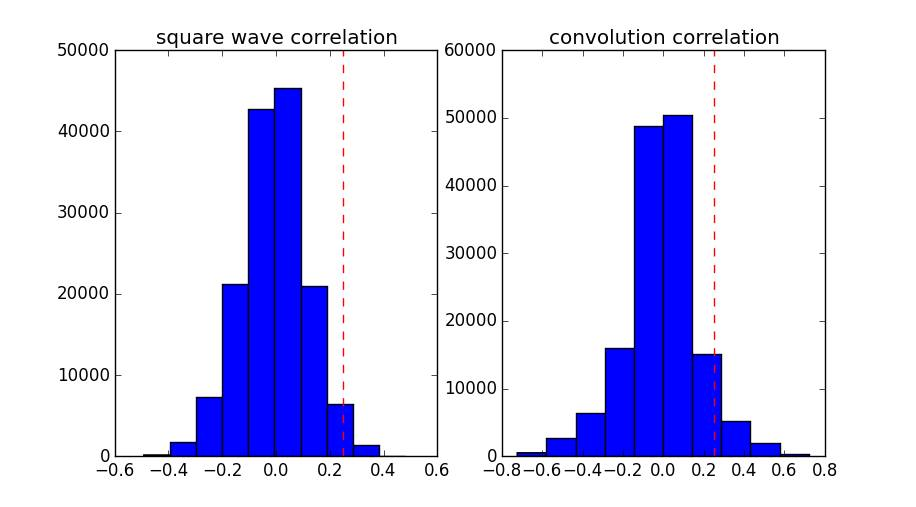
\includegraphics[width=16cm, height=8cm]{r_values_histogram.jpg}
\end{center}

Here, we want to compare the two types of analysis and decide on the better way
to find the activation regions. After calculating the correlations using both
square wave time course (SW method) and the convolved reference time course (CF
method) , we plot the histogram of r-values to understand the range and
the distribution of the correlation. With that information, we decided on
the threshold 0.20 to say whether a voxel is active or not active. We plot the
voxels which correlate to the reference waveform with $r > 0.20$ in red, so that
we can visually examine the activation level of the voxels in the brain. By comparing
the activated regions under square wave time course (left) and convolved time
course (right), we can clearly see that it is hard for SW method to detect the
activation while the CR method gives more reasonable and detailed
results.Therefore, we will use the convolved reference waveform for detecting
the task-dependent voxels in our future analysis.

\begin{center}
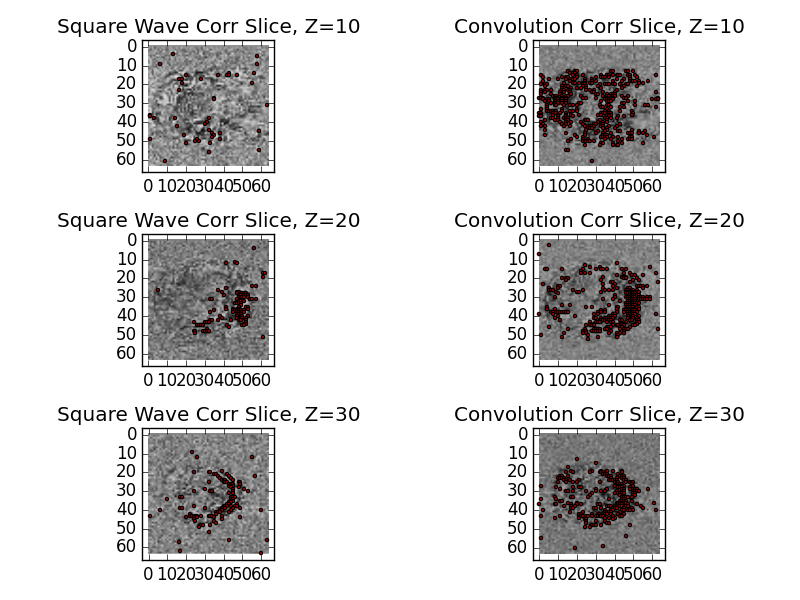
\includegraphics[width=12cm, height=12cm]{compare_correlations.png}
\end{center}

\subsection{Clustering with K-Means}

K-means clustering is an unsupervised technique which aims to partition n
observations into k clusters based on a feature set of n features. Each
observation is classified into the cluster with the nearest mean. In our case, n
is the number of voxels. k is chosen to be 5 although ideally, we should run
K-means with multiple k values \cite{venkataraman2009}. Clustering results
across the three runs of the same subject are merged together using a voting
algorithm \cite{dimitriadou2002}. We used three sets of features as described
below to obtain three sets of clustering results: (1) mean of BOLD signals over
time course for every voxel, (2) all signals in the time course for every voxel,
(3) all signals in the time course for every voxel, centered and normalized over
all signals in the corresponding time step. 

We do not involve the conditional file in the clustering. This is because the
underlying time courses are the same across methods as we compare across the
same subjects. Since Feature Set (1) only uses mean as a single feature, it
determines the clusters only based on intensity of the BOLD signals and can be
used a naive set of non-functional clusters (i.e. the other two or future
methods should deviate from this to reveal functional clusters). A comparison of
results across the three input feature sets is shown.

\begin{center}
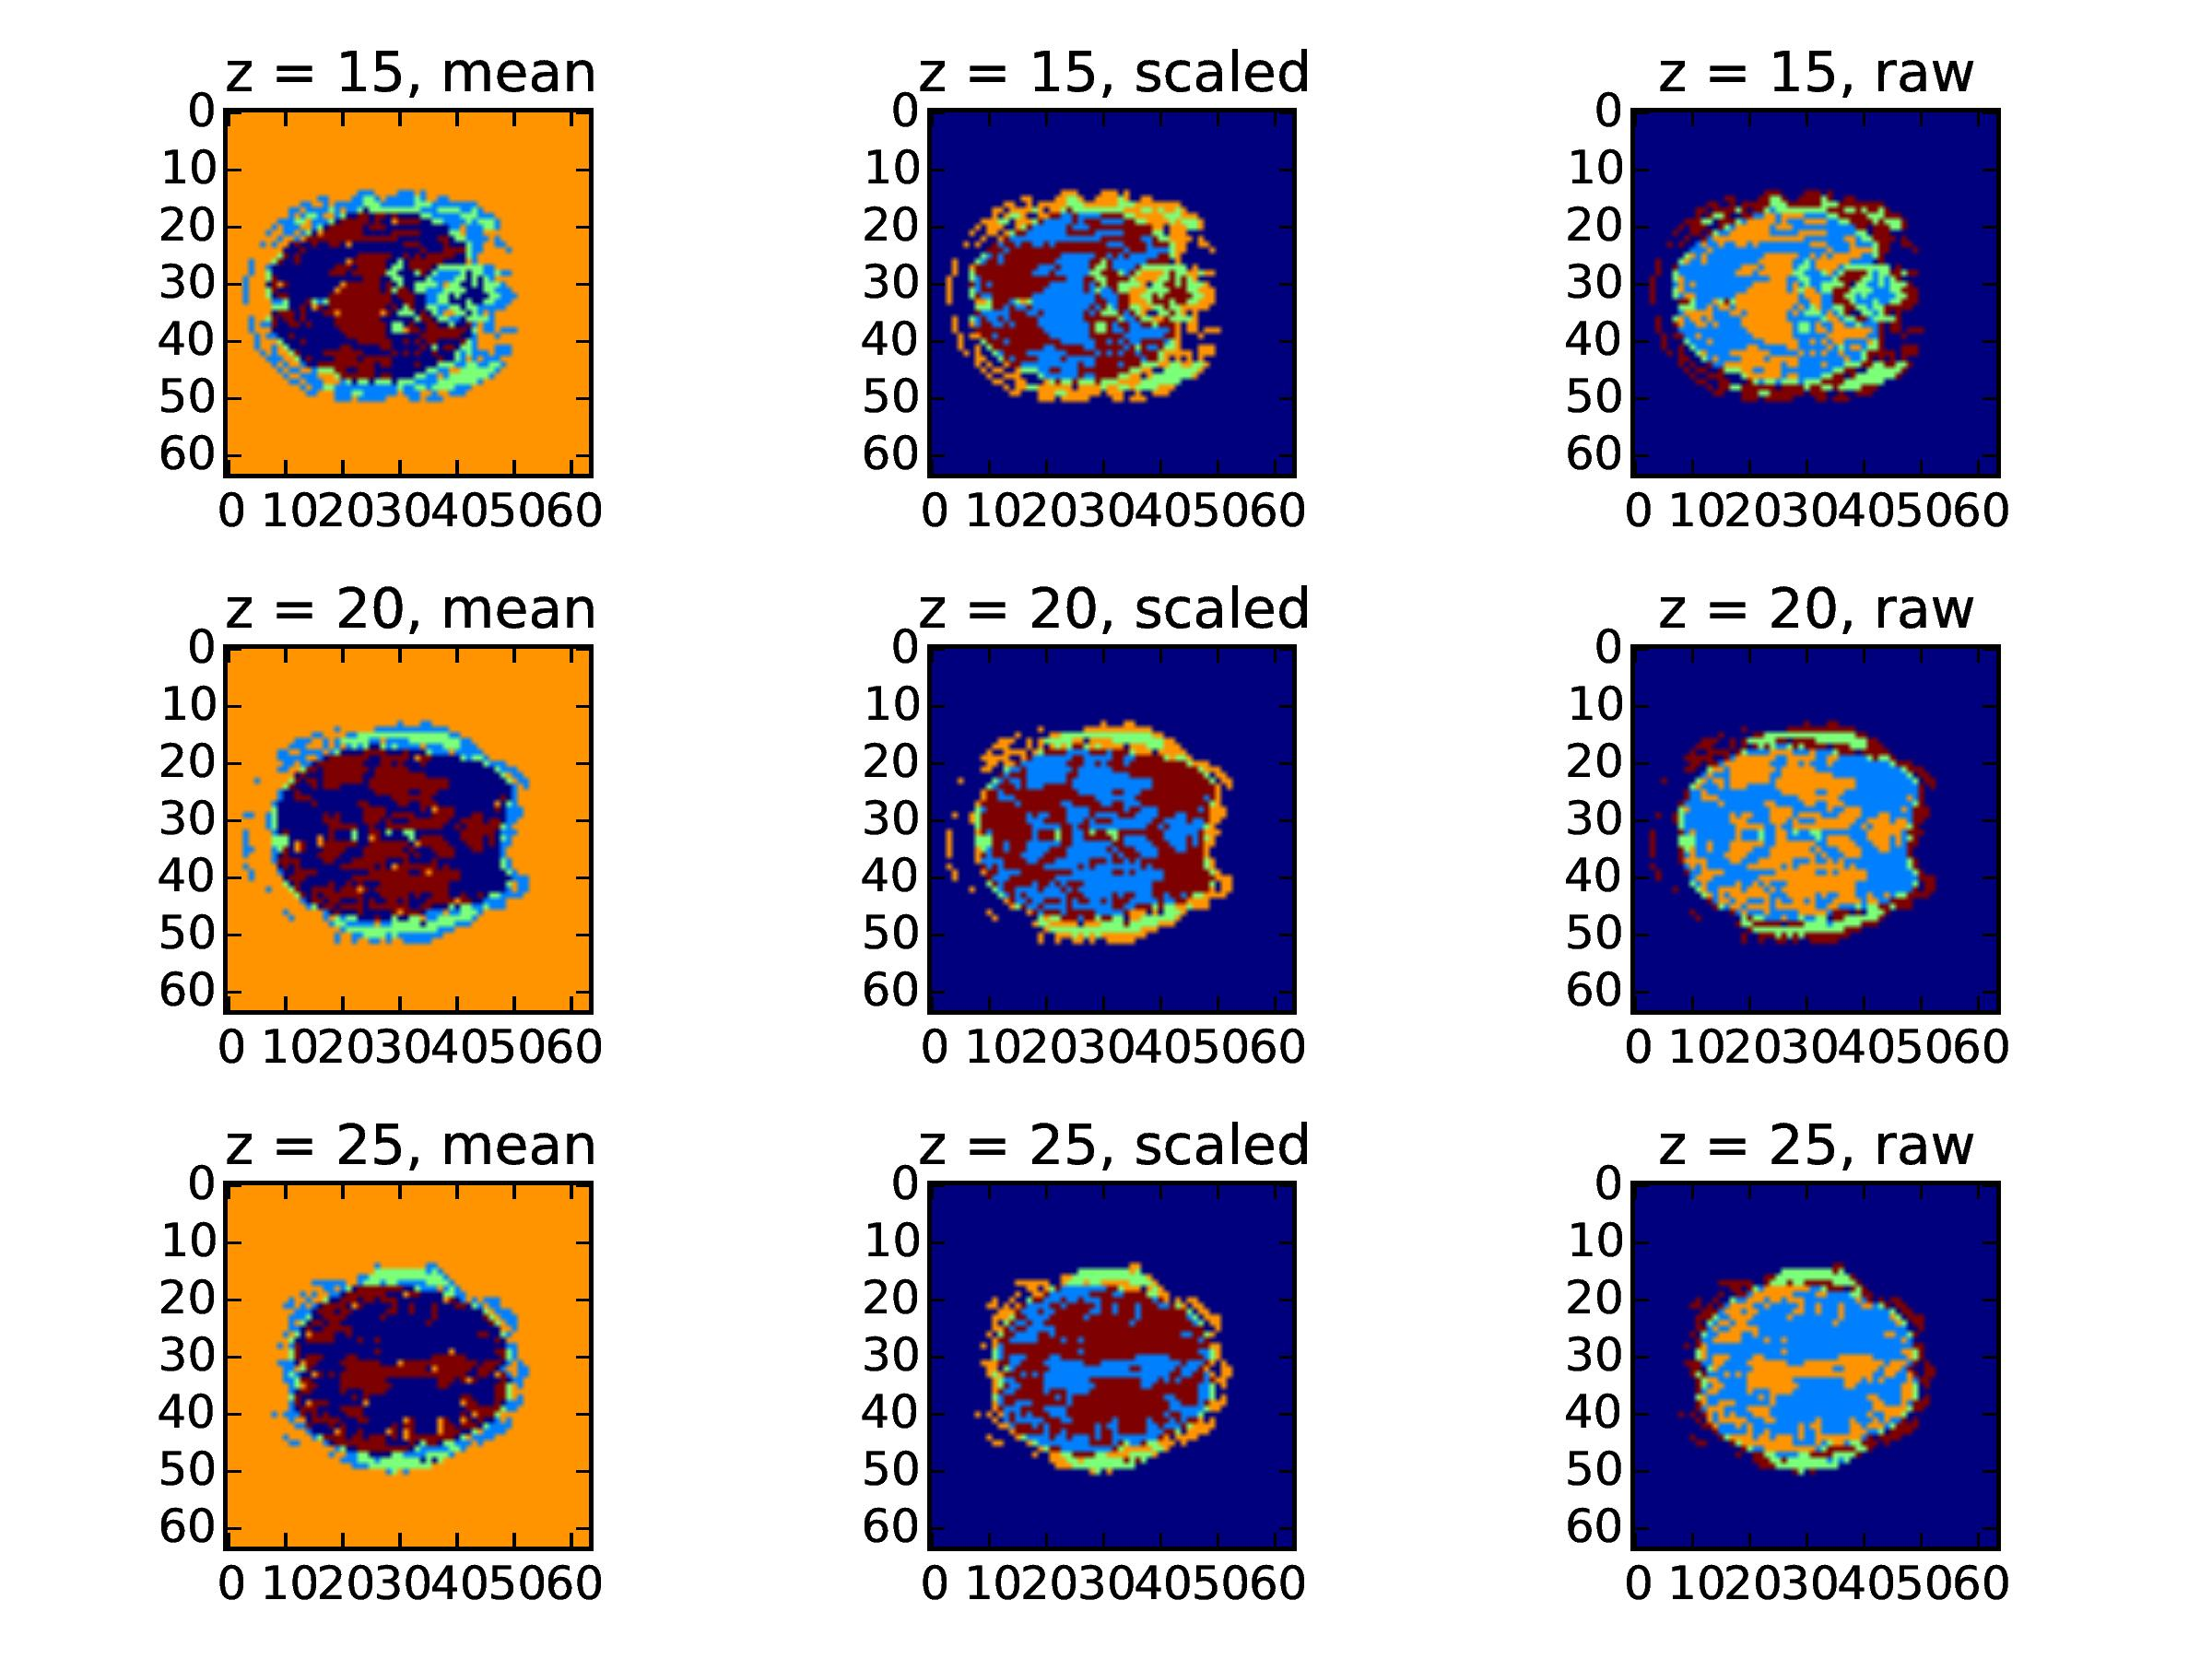
\includegraphics[width=12cm, height=12cm]{subject_across_methods.jpg}
\end{center}

Overall, basic and anatomical rather than functional clusters are revealed. For
example, the cerebral cortex is clustered together as well as the distinct
Thalamus-related region in the center of the brain.  Although there are visible
differences across subjects and runs, the differences across methods are almost
negligible. A scaled feature set has eliminated the intensity but does not
deviate from the naive clustering. The reason could be that there is too much
noise in the data. As an example, a drift term might be alone in determining the
clustering results. 

\subsection{Validation}

As we adopted a simple linear regression to fit our MRI data cross the predicted
neural time course, we need to check linear model assumptions before we conclude
validity of the model. One of the most important assumptions of linear model is
the normality of residuals.

Among the methods proposed to check normality, normal Q-Q plot is the most
commonly used. The Gaussian Q-Q plot compares residuals on the vertical axis
with a standard normal population on the horizontal axis. The linearity of the
points indicates normality. This method is straightforward and
intuitive. However, it has obvious weaknesses: (1) It can not evaluate multiple
vectors of residuals at same time; (2) there is no clear threshold to assert
normality. Therefore, it is not suitable for our normality test because we need
to check the normality on a per-voxel basis.

We used the Sharpiro-Wilk Test in which $H_0$ is $r_1,\dots ,r_n$ is normally
distributed. If the p-value we get from test statistic is less than the chosen
$\alpha$ level, then the null hypothesis is rejected and there is evidence that
the data tested are not from a normally distributed population.

Notice that we cannot naively compare all of these p-values individually with
$\alpha$, our type I error. Otherwise, our integrated type I error of test is
$\alpha^N$, vanishing as $N \rightarrow \infty$, which is too strict to check
multiple normality. Take the 11th subject as the example, if we just compare
p-values per voxel and $\alpha$ = 0.05, more than half of the test
($\frac{94397}{147456} =0.64$) will be rejected.

We have adopted several methods to handle this multiple comparison problem. 1)
Bonferroni procedure, in which reject the null if $p< \alpha/n$, where n is the
sample size. 2) Hochberg’s setup, in which order the p-values $p_1,\dots,p_n$ is
associate with corresponding hypothesis $H(1), \dots, H(n)$. Reject all
hypotheses $H(k) $ having $p(k)\leq \alpha/(n+1-k)$, where $ k=1,2,\dots,n$. 3)
Benjamini-Hochberg procedure, in which Order the p-values $P(1),P(2),\dots,P(n)$
and their associated hypothesis $H(1),\dots,H(n)$. Reject all hypotheses H(k)
having $P(k) \leq (k/n)\times \alpha $ ($k=1,\dots ,n$).

To be consistent with previous example, these three methods are also implemented
on the fMRI data of 11th subject: (1) with Bonferroni correction and outliers
removed, there are 32896 voxels out of 147456 are not normally distributed; (2)
with Hochberg's procedure and outliers removed, there are 4843 voxels out of
147456 that are not normally distributed; (3) with Benjamini-Hochberg's procedure and
outliers removed, there are 0 voxels out of 147456 that are not normally distributed.

\section{Discussion}

\subsection{Future Analysis}

\textbf{Extending and finetuning k-means}: We will continue working towards our goal of
revealing functional clustering of the brain. This can be done by:
 Improving the input features by inspecting and removing first principal
components of the datasets. This need to be done with care by visually
inspecting the principal components and consulting literature on the types and
characteristics of noise. One criterion of noise can be that the fluctuation has
a period clearly greater than the on-off cycle of the task. 

Improving input features by fitting the BOLD signals to a linear model and using
the residuals as input to K-means clustering. Using the same example above, a
drift term can be included in the design matrix so that it can be removed in the
residuals. This is the opposite of linear modelling to fit the data since in
this case, the aim is not to have a model to fit the data as best as possible
but to make use of the residuals in subsequent classification algorithms.

\begin{center}
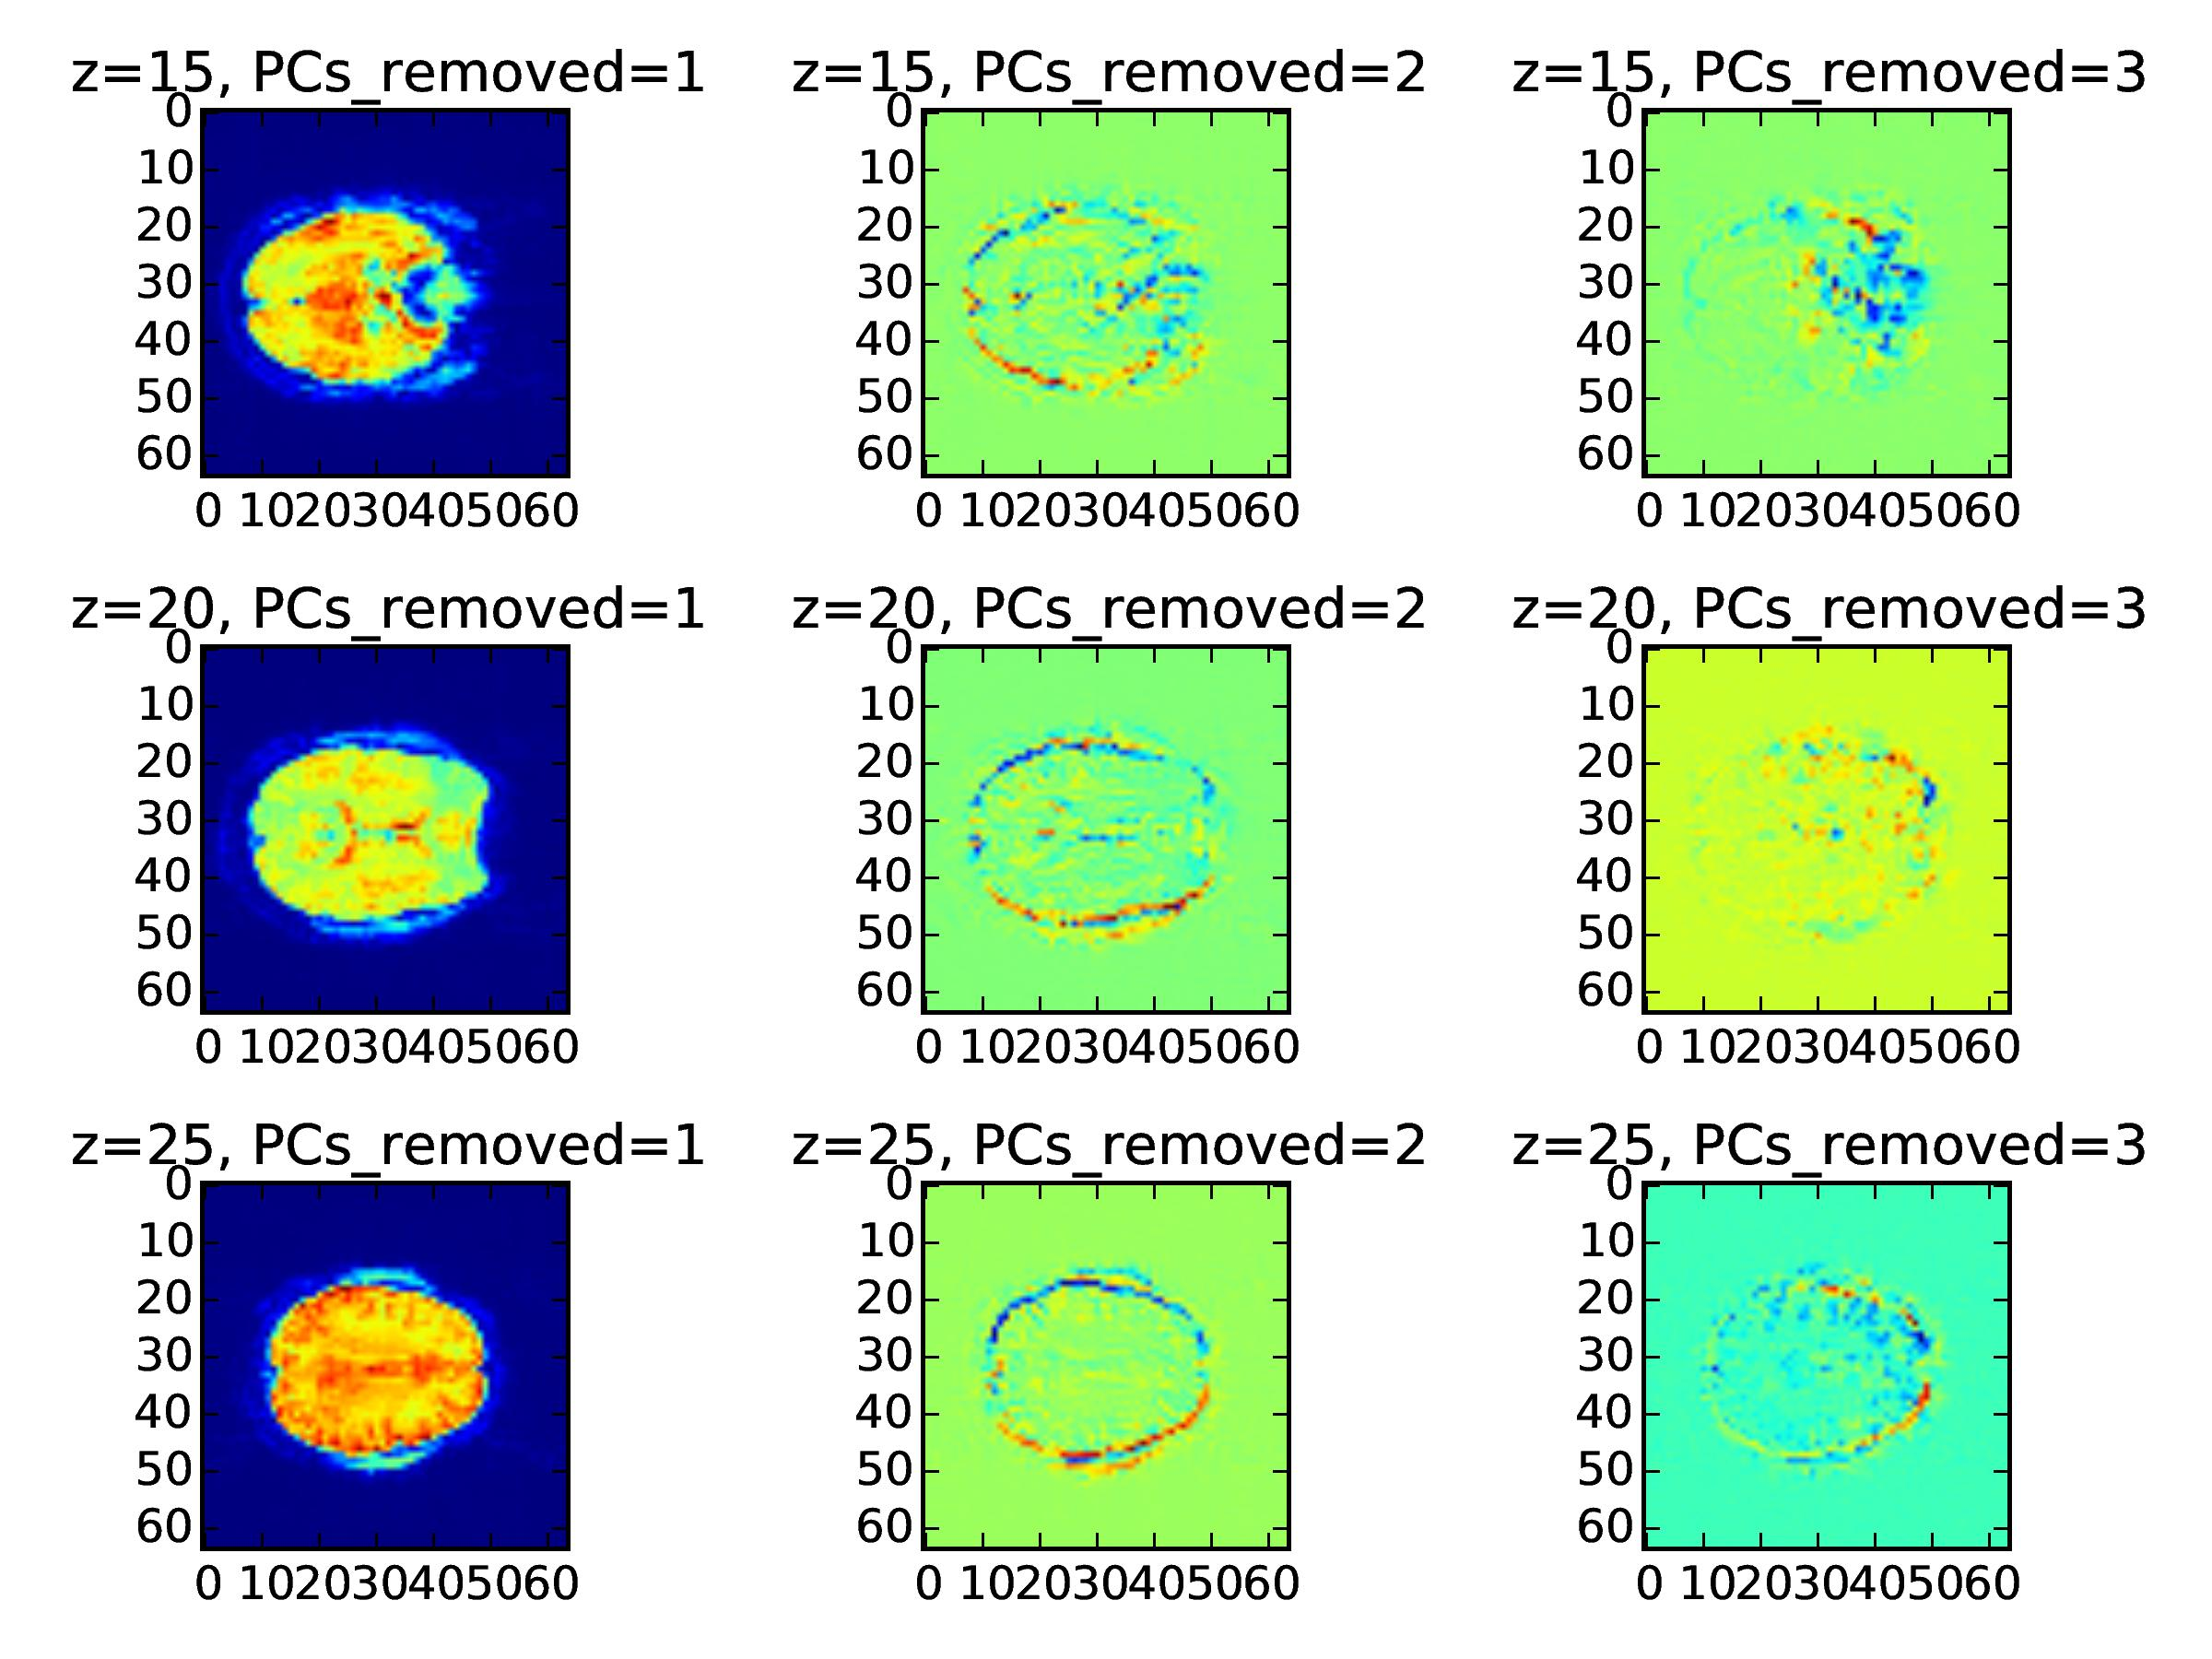
\includegraphics[width=12cm, height=12cm]{first_pcs_removed.jpg}
\end{center}

\textbf{Improving other analyses}: applying the same methods of noise reduction in
K-means in other analyses, 
such as correlations to refine the results and possibly make comparisons with
K-means. This is because both types of analysis serve to discover activation
regions. 

\textbf{Scaling analyses to make comparisons across different subject groups}: at this
stage, we focused on developing the scripts to analyze and make comparisons
within single subjects. From now on, we will apply the analyses across subject
groups in order to draw conclusions on differences in healthy and schizophrenia
subjects. To achieve this, some averaging techniques are necessary for
cross-group comparison. One example already mentioned is the merging algorithm
for K-means clustering. 

\textbf{Research other machine learning techniques to further
explore activation regions}: a greater variety of methods will allow us to reveal different insights about the data and make comparisons richer, giving us the freedom to explore and discuss the merits of different machine learning algorithms with respect to fMRI. 

\textbf{Talairach Space Transformation}: since one of our goals is to demonstrate activation regions revealed by the
datasets and compare those provided in the literature, we need to transform
coordinates to and back from Talairach space since most coordinates in
literature are provided in that space.

\subsection{Lessons Learned}

The dataset we use for our analysis is multi-layered and ambiguous in some sense. In our dataset, there are 3 runs for each subject as well as 7 condition files explaining the scan timeline for each run. In our analysis, the condition record we used has fractional seconds for scan duration (0.769951s), a very small proportion of the TR. In the example analysis seen in class, the durations we dealt with were always a multiple of the TR (2.5s). In this case, if we use the same TR as the scale, we would have to divide 0.769951 by 2.5 (around 0.30798) to fit the scale, the resulting convolution will deviate from the real scenario, causing bias. Therefore, we adopted the following strategy to tackle this problem: (1) rescaling data, converting from 2.5s to 0.1s as the unit; (2) in each 2.5s interval, choosing the median value to represent convolved data in that time interval; (3) convolving the data using the standard approach. This generates the convolved function we used in the analysis of correlations. 

Furthermore, the analysis done in the paper by Repovs \textit{et al.}�� is based on the Resting State dataset, in which they investigate the connectivity of the regions in the brain for patients and healthy controls \cite{repovs2012}. We tried to reproduce their result using the data; however, we encountered the problem of separating the resting state data from the rest of the BOLD signals. Consequently, it is important for us to find another potential, executable topic given the current dataset and develop a coherent rigorous statistical analysis.

\bibliography{report}

\end{document}
